\documentclass[11pt]{article}
\usepackage{array}
\usepackage{tabularx}
\usepackage{graphicx}
\title{
	\textbf{Data Mining Techniques 2013}
}

\author{Tobias Stahl \\ 10528199 \and Spyros Michaelides \\ 10523316 \and Ioannis Giounous Aivalis \\ s2538161 \and Francesco Stablum \\ 6200982}
\date{}
\usepackage{graphicx}
\begin{document}

\maketitle

\section{Introduction}



\section{Part 1}

In the initial section of the assignment an environment is constructed for the simulation of the agent, (the predator), and the prey. The environment is is a two dimensional toroidal grid in which, if an agent moves off the boundary of the side of the grid, he will appear at the opposite side of the board. The board has a size of 11 by 11 cells.\\
Both the predator and the prey move with a random policy inclusive of directions NORTH, SOUTH, WEST, EAST along with an option of staying still. While the predator has a 0.2 probability of taking any action, the prey has a probability 0.8 of staying in the same cell, and moves with a probability of only 0.05 in any direction.\\
The probability for action taken by the prey is changed when the predator will be standing in a neighboring cell, since the prey is not allowed to move into the cell of the predator. This will change the probability of the prey moving to 0.067 toward any of the remaining directions.\\
In order to find the average of moves it takes the predator to catch the prey a simulation of 100 runs is made. The resulting value for the average is 245.06 steps with a standard deviation of 205.836



\section{Part 2}

In the second part of the assignment, an iterative policy evaluation is used to determine the value for all possible states, using a discount factor of 0.8.\\
The value of a state is determined by summing the expected reward and value of all possible next states s' multiplied by the probability of actually moving into this state s'.\\
This is repeated as long as the policy keeps changing. Once this stops, the best policy is found.\\
The policy evaluation will stop once the change in values is smaller than threshold Theta, where Theta is 0.00000001.\\\\
Stated below are the values found by policy evaluation for sample states:\\\\
$\bullet$ Predator(0,0), Prey(5,5) $\Rightarrow 0.0089872$\\\\
$\bullet$ Predator(2,3), Prey(5,4) $\Rightarrow  0.2859599$\\\\
$\bullet$ Predator(2,10), Prey(10,0) $\Rightarrow  0.2859599$\\\\
$\bullet$ Predator(10,10), Prey(0,0) $\Rightarrow  1.9428952$\\\\
The algorithm took a total of 40 iterations to converge to the limit.


\section{Part 3}
In section three Policy Iteration has been implemented in order to find an optimal policy.
Once the all the states are evaluated using  Policy Evaluation (explained in part 2), a policy improvement algorithm is used to find the best action for the predator to take, regarding the reward to expect in the next state.\\
In order to do this the best action for each state is chosen by changing the probability of taking this action in this state to 1.0, while the rest of the actions in the state are reduced to a probability of 0. \\
Because of this change of probabilities the states need to be re-evaluated, leading to an iterative process until the policy is stable.


\subsection{Discount Factor ($\gamma$=0.8)}

For $\gamma$=0.1 the convergence of policy iteration occurs after 3 iterations. On the other hand the convergence of the policy in value iteration occurs after 11 iterations. Because of the small $\gamma$ not every state has a value over 0.001 as you can see in Table ~\ref{table:gamma=0.1} 

\begin{center}
\begin{table*}[ht]
{\small
\hfill{}
\begin{tabular}{c|c|c|c|c|c|c|c|c|c|c|c}
\textbf{} & \textbf{0} & \textbf{1} & \textbf{2} & \textbf{3} & \textbf{4} & \textbf{5} & \textbf{6} & \textbf{7} & \textbf{8} & \textbf{9} & \textbf{10}\\
	\hline
\textbf(0) & 5.5047017 & 6.7167281 &
8.4475634 & 10.5604615 & 13.1073657 & 15.3929361 & 12.9437720 & 10.5243359 & 8.5624895 & 6.9303996 & 5.5557952\\
\textbf(1) & 6.7972655 & 8.4475634 & 10.5604615 & 13.1073657 & 16.3471023 & 19.5153974 & 16.2827410 & 12.9437720 & 10.5082463 & 8.4611194 & 6.8008181\\
\textbf(2) & 8.4727784 & 10.4812716 & 13.0996596 & 16.3435817 & 20.3389022 & 24.7364728 & 19.9305513 & 16.0689053 & 13.0275927 & 10.3692282 & 8.4276146\\
\textbf(3) & 10.4812716 & 13.0996596 & 16.3435817 & 20.3389022 & 24.7364728 & 31.4772727 & 24.7364728 & 19.9305513 & 16.0689053 & 13.0275927 & 10.3692282\\
\textbf(4) & 12.1034383 & 15.2339321 & 19.4022351 & 24.7107438 & 31.4772727 & 39.9999999 & 31.4772727 & 24.7107438 & 19.4022351 & 15.2339321 & 12.1034383\\
\textbf(5) & 15.2339321 & 19.4022351 & 24.7107438 & 31.4772727 & 39.9999999 & 39.9999999 & 39.9999999 & 31.4772727 & 24.7107438 & 19.4022351 & 15.2339321\\
\textbf(6) & 12.1034383 & 15.2339321 & 19.4022351 & 24.7107438 & 31.4772727 & 39.9999999 & 31.4772727 & 24.7107438 & 19.4022351 & 15.2339321 & 12.1034383\\
\textbf(7) & 10.4869380 & 13.1009056 & 16.3435817 & 20.3389022 & 24.7364728 & 31.4772727 & 24.7364728 & 19.9621538 & 16.2775954 & 12.8978728 & 10.3482308\\
\textbf(8) & 8.47679982 & 10.4869380 & 13.1009056 & 16.3435817 & 20.3389022 & 24.7364728 & 19.9621538 & 16.2775954 & 12.8978728 & 10.3482308 & 8.44741514\\
\textbf(9) & 6.87213440 & 8.46853140 & 10.5392768 & 13.1072130 & 16.3474741 & 19.5156461 & 16.3261473 & 13.0717223 & 10.5183736 & 8.38762582 & 6.85502400\\
\textbf(10) & 5.5706362 & 6.79892487 & 8.46853140 & 10.5392768 & 13.1072130 & 15.4040036 & 13.0717223 & 10.5183736 & 8.38762582 & 6.78326202 & 5.55840548\\
\end{tabular}}
\hfill{}
\caption{Values of all states at which the prey is located at (5,5) with a discount factor of ($\gamma$=0.8), convergence after 16 iterations.}
\label{table:gamma=0.8}
\end{table*}
\end{center}



\begin{center}
\begin{table*}[ht]
{\small
\hfill{}
\begin{tabular}{c|c|c}
\textbf{Discount Factor} & \textbf{Policy Iteration} & \textbf{Value Iteration}\\
	\hline
0.1 & 11 & 0\\
0.5 & 14 & 0\\
0.7 & 15 & 0\\
0.9 & 22 & 0\\
\end{tabular}}
\hfill{}
\caption{Number of iterations for different discount factors.}
\label{table:gamma=0.8}
\end{table*}
\end{center}

\section{Value Iteration}
In section 4, value iteration is implemented. The difference between value iteration and policy iteration, is that "Value iteration effectively combines, in each of its sweeps, one sweep of policy evaluation and one sweep of policy improvement." \cite{barto1}\\
A plot of all $\gamma$ between 0 and 1 can be seen in Figure ~\ref{plot}.
\begin{figure}
\centering
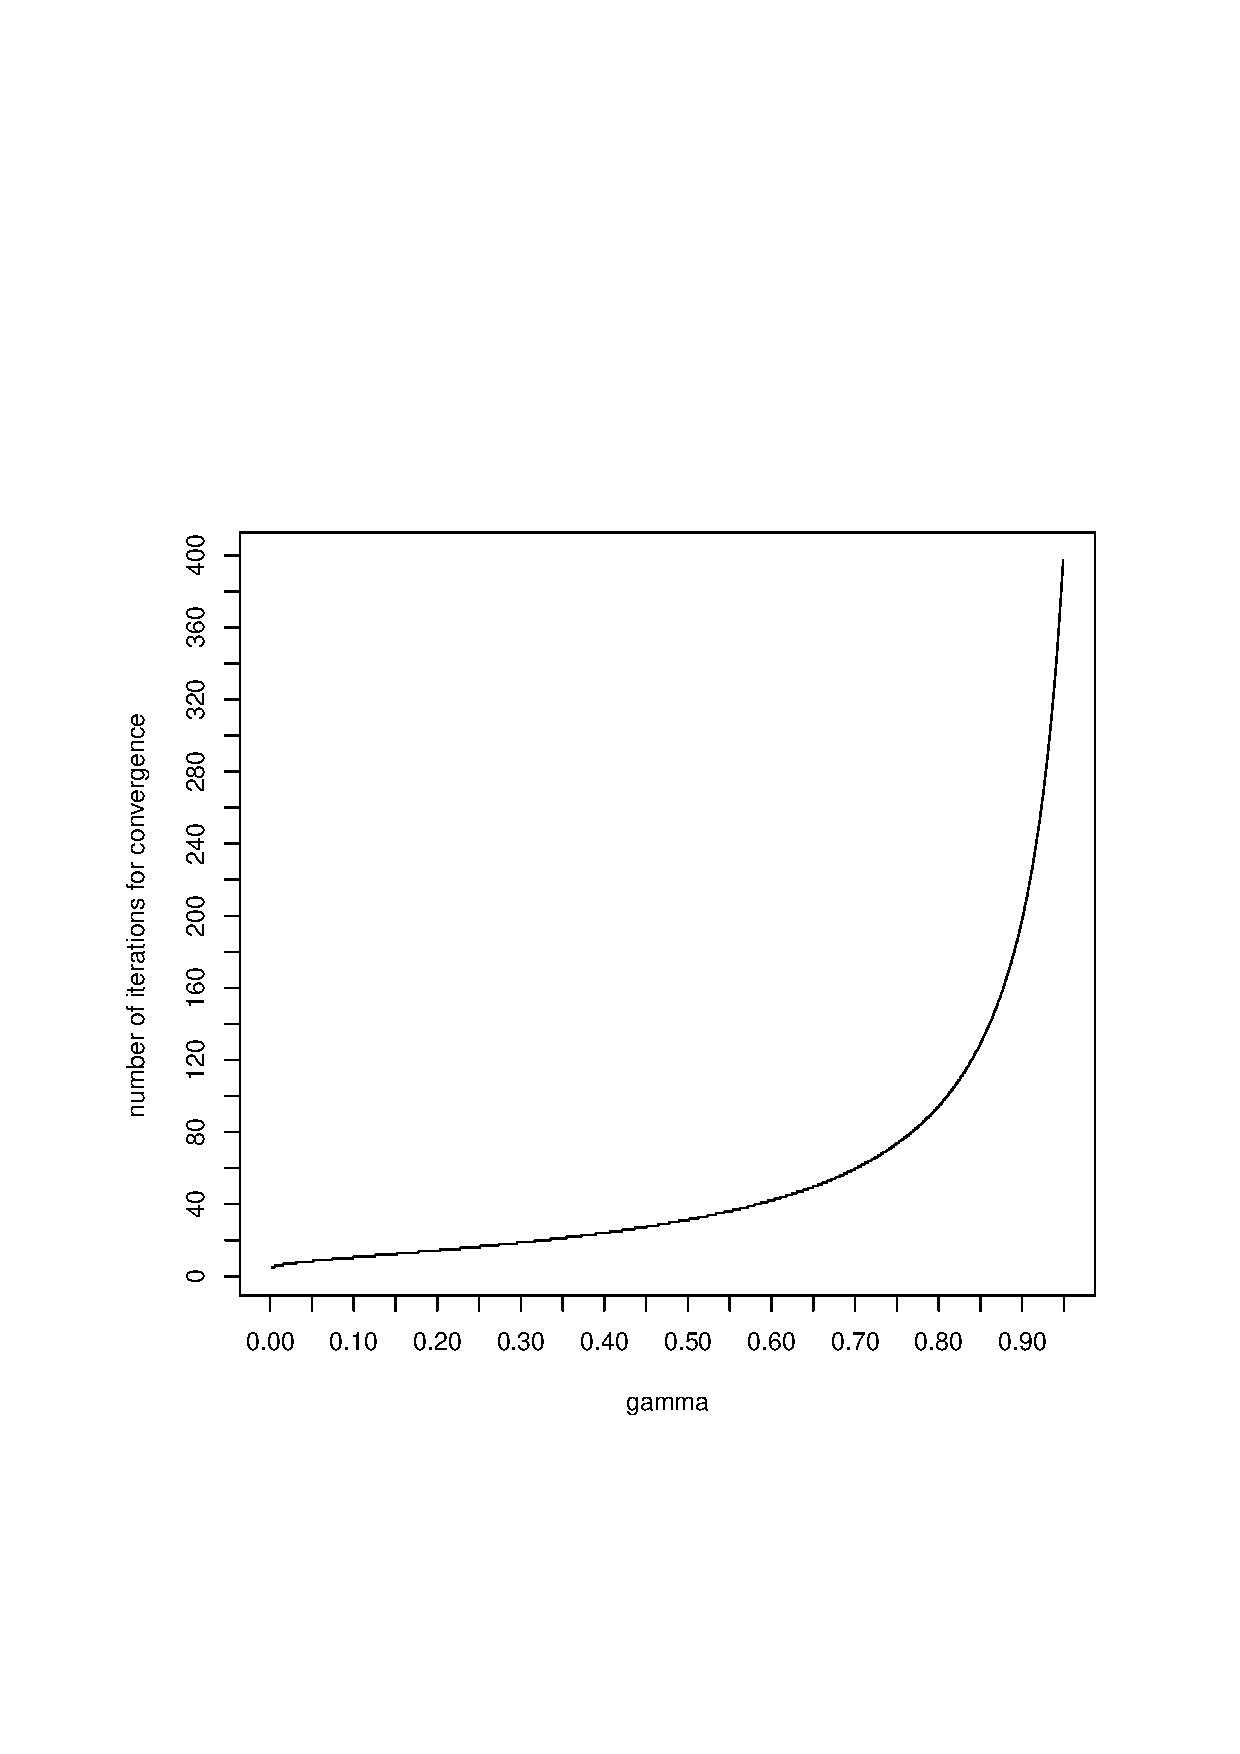
\includegraphics[scale=0.8]{a14.png}
\caption{Plot of $\gamma$ and their number of iterations to converge}
\label{plot}
\end{figure}






\begin{thebibliography}{7}

\bibitem{barto1} http://webdocs.cs.ualberta.ca/~sutton/book/ebook/node44.html


\end{thebibliography}
\end{document}
